\documentclass{article}
\usepackage{graphicx}
\usepackage{tikz}
\usetikzlibrary{shapes.geometric, arrows, positioning, fit}

\title{Assignment 3\\ `Whisper'\\ System Design}
\author{
    Joakim Tollefsen Johannesen\\
    \texttt{joakimtj@hiof.no}
    \and
    Niklas Berby\\
    \texttt{niklab@hiof.no}
}
\date{2024}

\begin{document}
\maketitle
\section{Technical Structure}
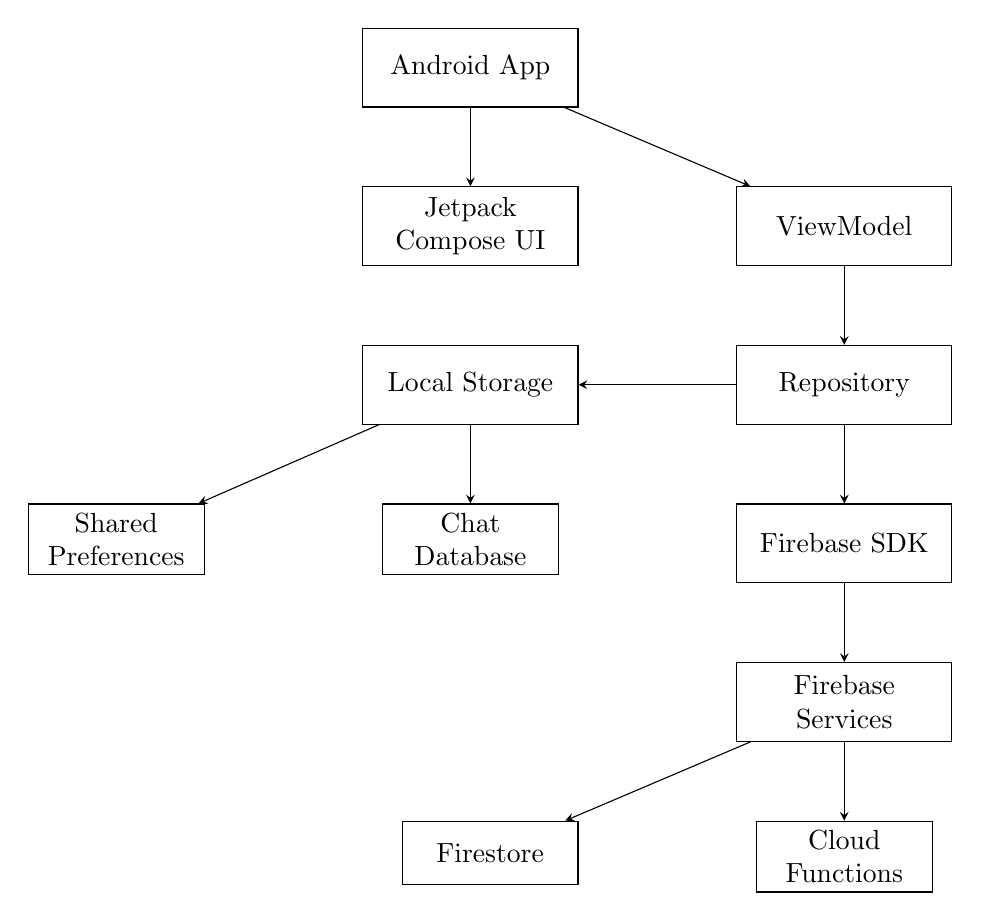
\begin{tikzpicture}[
    node distance = 1cm and 2cm,
    box/.style = {rectangle, draw, text width=2.5cm, text centered, minimum height=1cm},
    smallbox/.style = {rectangle, draw, text width=2cm, text centered, minimum height=0.8cm},
    arrow/.style = {->, >=stealth}
]

% Define nodes
\node[box] (app) {Android App};
\node[box, below=of app] (ui) {Jetpack Compose UI};
\node[box, right=of ui] (viewmodel) {ViewModel};
\node[box, below=of viewmodel] (repository) {Repository};
\node[box, below=of repository] (firebase) {Firebase SDK};
\node[box, below=of firebase] (services) {Firebase Services};
\node[smallbox, below left=of services] (firestore) {Firestore};
\node[smallbox, below=of services] (functions) {Cloud Functions};
\node[box, left=of repository] (local) {Local Storage};
\node[smallbox, below left=of local] (prefs) {Shared Preferences};
\node[smallbox, below=of local] (room) {Chat Database};

% Draw arrows
\draw[arrow] (app) -- (ui);
\draw[arrow] (app) -- (viewmodel);
\draw[arrow] (viewmodel) -- (repository);
\draw[arrow] (repository) -- (firebase);
\draw[arrow] (firebase) -- (services);
\draw[arrow] (services) -- (firestore);
\draw[arrow] (services) -- (functions);
\draw[arrow] (repository) -- (local);
\draw[arrow] (local) -- (prefs);
\draw[arrow] (local) -- (room);

\end{tikzpicture}
\end{document}